\chapter{Methodology}

\section{Introduction}
This chapter presents the design and architectural implementation of the proposed
detector for very small human targets in aerial search-and-rescue imagery. The
methodology treats the task as a resolution-and-attention problem: the targets of
interest are frequently smaller than the finest detection cell of a standard
one-stage detector, and they sit in heavy background clutter. The proposed model
therefore modifies the YOLO11m baseline (reviewed in Chapter~II) in exactly two
places: a Convolutional Block Attention Module (CBAM) replaces the C2PSA attention
block at the end of the backbone, and the neck and head are extended with a
stride-4 (P2) detection scale. A third component, a bidirectional state-space
(Mamba) neck block, was explored under the same protocol and is reported honestly
as a negative result. Rather than adopting a single fixed architecture, the model
is developed through an \emph{additive ablation}: one architectural change is
introduced at a time so that the contribution of each component can be attributed
independently. The following sections give the system overview, the layer-level
architecture, the novelties and their rationale, the loss design, and the
inference-time enhancement procedures evaluated in Chapter~IV.

\section{System Architecture Overview}
The complete pipeline is shown in Figure~\ref{fig:framework}. Given an aerial
image, the system letterbox-resizes it to $640 \times 640$, extracts multi-scale
features with the YOLO11m backbone, refines the deepest features with CBAM,
fuses all scales in a PAN--FPN neck extended down to stride~4, and decodes boxes
at four scales before non-maximum suppression (NMS) produces the final human
detections.

\begin{figure}[H]
  \centering
  % ============================================================================
%  fig_system_overview.tex -- high-level schematic of the proposed pipeline.
%  Sample-thesis Figure-3.1 style: six stages in a two-row snake flow.
%  Colours follow the house palette; the two modifications are red-accented.
%  Needs \usepackage{tikz} (loaded in thesisstyle.sty).
%  Include with:  % ============================================================================
%  fig_system_overview.tex -- high-level schematic of the proposed pipeline.
%  Sample-thesis Figure-3.1 style: six stages in a two-row snake flow.
%  Colours follow the house palette; the two modifications are red-accented.
%  Needs \usepackage{tikz} (loaded in thesisstyle.sty).
%  Include with:  % ============================================================================
%  fig_system_overview.tex -- high-level schematic of the proposed pipeline.
%  Sample-thesis Figure-3.1 style: six stages in a two-row snake flow.
%  Colours follow the house palette; the two modifications are red-accented.
%  Needs \usepackage{tikz} (loaded in thesisstyle.sty).
%  Include with:  \input{tikz/fig_system_overview}
% ============================================================================
\definecolor{soBlueFill}{HTML}{DAE8FC}
\definecolor{soBlueStroke}{HTML}{6C8EBF}
\definecolor{soGreenFill}{HTML}{D5E8D4}
\definecolor{soGreenStroke}{HTML}{82B366}
\definecolor{soOrangeFill}{HTML}{FFE6CC}
\definecolor{soOrangeStroke}{HTML}{D79B00}
\definecolor{soPurpleFill}{HTML}{E1D5E7}
\definecolor{soPurpleStroke}{HTML}{9673A6}
\definecolor{soRed}{HTML}{FF0000}
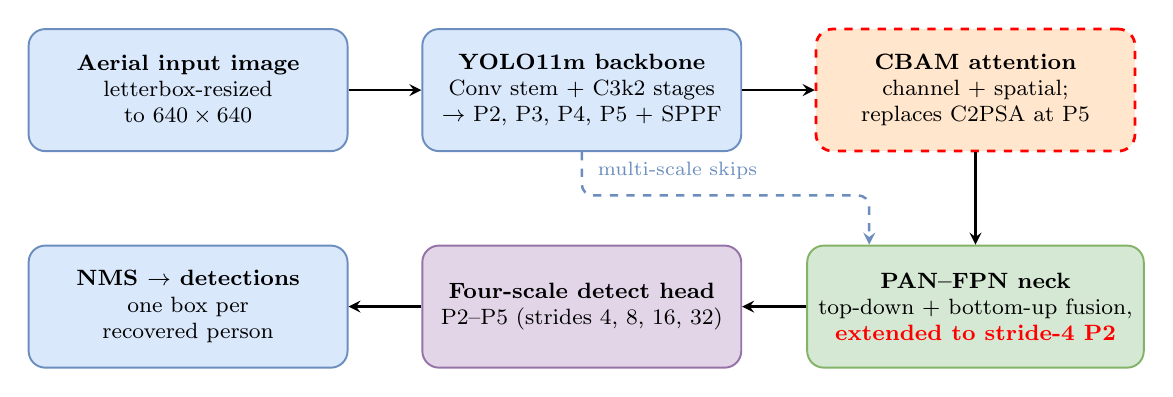
\begin{tikzpicture}[
  font=\footnotesize,
  stage/.style={rounded corners=6pt, draw, align=center,
                minimum width=4.05cm, minimum height=1.55cm,
                inner sep=4pt, line width=0.7pt},
  flow/.style={-{stealth}, line width=0.9pt}
]
  % ---- row 1 (left to right) ----
  \node[stage, fill=soBlueFill, draw=soBlueStroke] (inp) at (0,0)
        {\textbf{Aerial input image}\\letterbox-resized\\to $640\times640$};
  \node[stage, fill=soBlueFill, draw=soBlueStroke] (bb) at (5.0,0)
        {\textbf{YOLO11m backbone}\\Conv stem + C3k2 stages\\$\rightarrow$ P2, P3, P4, P5 + SPPF};
  \node[stage, fill=soOrangeFill, draw=soRed, dashed, line width=1.0pt] (cbam) at (10.0,0)
        {\textbf{CBAM attention}\\channel + spatial;\\replaces C2PSA at P5};

  % ---- row 2 (right to left) ----
  \node[stage, fill=soGreenFill, draw=soGreenStroke] (neck) at (10.0,-2.75)
        {\textbf{PAN--FPN neck}\\top-down + bottom-up fusion,\\\textcolor{soRed}{\textbf{extended to stride-4 P2}}};
  \node[stage, fill=soPurpleFill, draw=soPurpleStroke] (head) at (5.0,-2.75)
        {\textbf{Four-scale detect head}\\P2--P5 (strides 4, 8, 16, 32)};
  \node[stage, fill=soBlueFill, draw=soBlueStroke] (out) at (0,-2.75)
        {\textbf{NMS $\rightarrow$ detections}\\one box per\\recovered person};

  % ---- flow arrows (snake) ----
  \draw[flow] (inp) -- (bb);
  \draw[flow] (bb) -- (cbam);
  \draw[flow] (cbam) -- (neck);
  \draw[flow] (neck) -- (head);
  \draw[flow] (head) -- (out);

  % ---- skip connections annotation (orthogonal, through the row gap) ----
  \draw[flow, dashed, soBlueStroke, rounded corners=4pt]
        (bb.south) -- ++(0,-0.55)
        node[pos=1, above right=2pt, font=\scriptsize, text=soBlueStroke]
        {multi-scale skips}
        -| ([xshift=-1.35cm]neck.north);
\end{tikzpicture}

% ============================================================================
\definecolor{soBlueFill}{HTML}{DAE8FC}
\definecolor{soBlueStroke}{HTML}{6C8EBF}
\definecolor{soGreenFill}{HTML}{D5E8D4}
\definecolor{soGreenStroke}{HTML}{82B366}
\definecolor{soOrangeFill}{HTML}{FFE6CC}
\definecolor{soOrangeStroke}{HTML}{D79B00}
\definecolor{soPurpleFill}{HTML}{E1D5E7}
\definecolor{soPurpleStroke}{HTML}{9673A6}
\definecolor{soRed}{HTML}{FF0000}
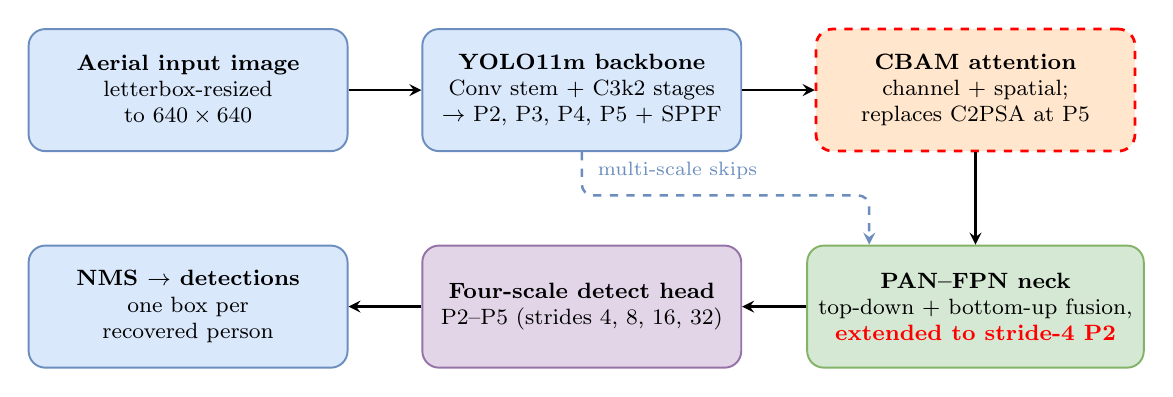
\begin{tikzpicture}[
  font=\footnotesize,
  stage/.style={rounded corners=6pt, draw, align=center,
                minimum width=4.05cm, minimum height=1.55cm,
                inner sep=4pt, line width=0.7pt},
  flow/.style={-{stealth}, line width=0.9pt}
]
  % ---- row 1 (left to right) ----
  \node[stage, fill=soBlueFill, draw=soBlueStroke] (inp) at (0,0)
        {\textbf{Aerial input image}\\letterbox-resized\\to $640\times640$};
  \node[stage, fill=soBlueFill, draw=soBlueStroke] (bb) at (5.0,0)
        {\textbf{YOLO11m backbone}\\Conv stem + C3k2 stages\\$\rightarrow$ P2, P3, P4, P5 + SPPF};
  \node[stage, fill=soOrangeFill, draw=soRed, dashed, line width=1.0pt] (cbam) at (10.0,0)
        {\textbf{CBAM attention}\\channel + spatial;\\replaces C2PSA at P5};

  % ---- row 2 (right to left) ----
  \node[stage, fill=soGreenFill, draw=soGreenStroke] (neck) at (10.0,-2.75)
        {\textbf{PAN--FPN neck}\\top-down + bottom-up fusion,\\\textcolor{soRed}{\textbf{extended to stride-4 P2}}};
  \node[stage, fill=soPurpleFill, draw=soPurpleStroke] (head) at (5.0,-2.75)
        {\textbf{Four-scale detect head}\\P2--P5 (strides 4, 8, 16, 32)};
  \node[stage, fill=soBlueFill, draw=soBlueStroke] (out) at (0,-2.75)
        {\textbf{NMS $\rightarrow$ detections}\\one box per\\recovered person};

  % ---- flow arrows (snake) ----
  \draw[flow] (inp) -- (bb);
  \draw[flow] (bb) -- (cbam);
  \draw[flow] (cbam) -- (neck);
  \draw[flow] (neck) -- (head);
  \draw[flow] (head) -- (out);

  % ---- skip connections annotation (orthogonal, through the row gap) ----
  \draw[flow, dashed, soBlueStroke, rounded corners=4pt]
        (bb.south) -- ++(0,-0.55)
        node[pos=1, above right=2pt, font=\scriptsize, text=soBlueStroke]
        {multi-scale skips}
        -| ([xshift=-1.35cm]neck.north);
\end{tikzpicture}

% ============================================================================
\definecolor{soBlueFill}{HTML}{DAE8FC}
\definecolor{soBlueStroke}{HTML}{6C8EBF}
\definecolor{soGreenFill}{HTML}{D5E8D4}
\definecolor{soGreenStroke}{HTML}{82B366}
\definecolor{soOrangeFill}{HTML}{FFE6CC}
\definecolor{soOrangeStroke}{HTML}{D79B00}
\definecolor{soPurpleFill}{HTML}{E1D5E7}
\definecolor{soPurpleStroke}{HTML}{9673A6}
\definecolor{soRed}{HTML}{FF0000}
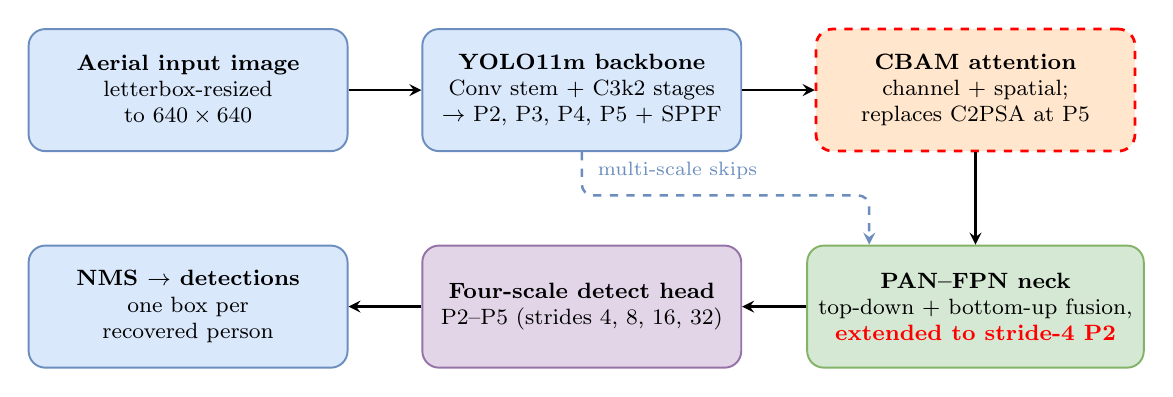
\begin{tikzpicture}[
  font=\footnotesize,
  stage/.style={rounded corners=6pt, draw, align=center,
                minimum width=4.05cm, minimum height=1.55cm,
                inner sep=4pt, line width=0.7pt},
  flow/.style={-{stealth}, line width=0.9pt}
]
  % ---- row 1 (left to right) ----
  \node[stage, fill=soBlueFill, draw=soBlueStroke] (inp) at (0,0)
        {\textbf{Aerial input image}\\letterbox-resized\\to $640\times640$};
  \node[stage, fill=soBlueFill, draw=soBlueStroke] (bb) at (5.0,0)
        {\textbf{YOLO11m backbone}\\Conv stem + C3k2 stages\\$\rightarrow$ P2, P3, P4, P5 + SPPF};
  \node[stage, fill=soOrangeFill, draw=soRed, dashed, line width=1.0pt] (cbam) at (10.0,0)
        {\textbf{CBAM attention}\\channel + spatial;\\replaces C2PSA at P5};

  % ---- row 2 (right to left) ----
  \node[stage, fill=soGreenFill, draw=soGreenStroke] (neck) at (10.0,-2.75)
        {\textbf{PAN--FPN neck}\\top-down + bottom-up fusion,\\\textcolor{soRed}{\textbf{extended to stride-4 P2}}};
  \node[stage, fill=soPurpleFill, draw=soPurpleStroke] (head) at (5.0,-2.75)
        {\textbf{Four-scale detect head}\\P2--P5 (strides 4, 8, 16, 32)};
  \node[stage, fill=soBlueFill, draw=soBlueStroke] (out) at (0,-2.75)
        {\textbf{NMS $\rightarrow$ detections}\\one box per\\recovered person};

  % ---- flow arrows (snake) ----
  \draw[flow] (inp) -- (bb);
  \draw[flow] (bb) -- (cbam);
  \draw[flow] (cbam) -- (neck);
  \draw[flow] (neck) -- (head);
  \draw[flow] (head) -- (out);

  % ---- skip connections annotation (orthogonal, through the row gap) ----
  \draw[flow, dashed, soBlueStroke, rounded corners=4pt]
        (bb.south) -- ++(0,-0.55)
        node[pos=1, above right=2pt, font=\scriptsize, text=soBlueStroke]
        {multi-scale skips}
        -| ([xshift=-1.35cm]neck.north);
\end{tikzpicture}

  \caption{High-level schematic of the proposed detection pipeline.}
  \label{fig:framework}
\end{figure}

The workflow has three phases:
\begin{itemize}
  \item \textbf{Feature extraction and attention.} The backbone produces feature
  maps at strides 2--32 (P1--P5). At the deepest level, CBAM applies channel
  attention followed by spatial attention, re-weighting the 512-channel P5
  features so that human-shaped responses are emphasised over debris, water, and
  vegetation before any fusion happens.
  \item \textbf{Multi-scale fusion with a P2 extension.} The neck runs the usual
  top-down and bottom-up passes, but the top-down pass continues one level
  further than the standard design: it upsamples to stride~4 and fuses the
  high-resolution backbone P2 features, producing a $160 \times 160$ map whose
  cells cover only $4 \times 4$ input pixels.
  \item \textbf{Four-scale decoding.} The head predicts boxes at strides 4, 8,
  16, and 32; NMS merges overlapping candidates so that clusters of nearby
  people are kept as separate detections.
\end{itemize}

\section{Proposed System Architecture}
Figure~\ref{fig:fullarch} traces the complete data flow of the proposed
detector on a real C2A scene. An input image enters at the top left and passes
through the YOLO11m backbone, which produces feature maps at five decreasing
resolutions from P1 to P5. At the deepest level the CBAM block, drawn in
orange, replaces the original C2PSA attention and re-weights the P5 features
before any fusion happens. The PAN--FPN neck then fuses the scales in a
top-down and a bottom-up pass, and the fusion is carried one level further than
the standard design so that a high-resolution stride-4 (P2) branch is produced.
The four fused scales feed a single detection head, and non-maximum suppression
returns one box per recovered person. The image insets placed around the
diagram are the model's own signals on this scene, read as input, CBAM
attention map, P2 feature response, and final detections; they show that the
attention concentrates on human-shaped regions and that the P2 branch responds
to the smallest scattered figures.

\begin{figure}[H]
  \centering
  \figorplaceholder{figures/figures_png_format/cbam_p2_architecture.png}{10.5cm}
  \caption{Layer-level architecture of the proposed detector on a real C2A scene.}
  \label{fig:fullarch}
\end{figure}

Table~\ref{tab:layers} lists the same architecture one layer at a time, so the
figure can be reproduced exactly; it is the verbatim training configuration
used in every experiment. The backbone, layers 0 to 9, halves the spatial
resolution at each stage while raising the channel count, and layers 1 to 6 are
marked as skip sources because the neck reuses their outputs later. The two
bold rows are the elements this work changes: CBAM at layer~10, which replaces
the C2PSA block at the end of the backbone at no increase in resolution, and
the added P2 branch at layers 17 to 19, which upsamples to a $160\times160$ map
and fuses the high-resolution backbone features. The head at layer~29 reads the
four fused scales at strides 4, 8, 16, and 32, one detection level more than the
stock three-scale head. The channel counts are the values realised at the
YOLO11m width of 1.0, channel cap of 512, and depth of 0.5.

{\small
\setlength{\tabcolsep}{7pt}
\renewcommand{\arraystretch}{1.3}
\begin{longtable}{@{}c l l l@{}}
  \caption{Layer configuration of the proposed detector at 640-px input.}
  \label{tab:layers}\\
  \toprule
  \textbf{Layers} & \textbf{Module (arguments)} & \textbf{Output} & \textbf{Role} \\
  \midrule
  \endfirsthead
  \multicolumn{4}{@{}l}{\itshape Table~\ref{tab:layers} (Continued)}\\[2pt]
  \toprule
  \textbf{Layers} & \textbf{Module (arguments)} & \textbf{Output} & \textbf{Role} \\
  \midrule
  \endhead
  \endfoot
  \bottomrule
  \endlastfoot
    0      & Conv(64, $3{\times}3$, s2)   & $320^2 \times 64$   & stem, P1/2 \\
    1--2   & Conv(128, s2); C3k2(256)     & $160^2 \times 256$  & P2/4 (skip source) \\
    3--4   & Conv(256, s2); C3k2(512)     & $80^2 \times 512$   & P3/8 (skip source) \\
    5--6   & Conv(512, s2); C3k2(512)     & $40^2 \times 512$   & P4/16 (skip source) \\
    7--9   & Conv(512, s2); C3k2; SPPF    & $20^2 \times 512$   & P5/32 \\
    \textbf{10} & \textbf{CBAM ($r{=}16$, $k{=}7$)} & $20^2 \times 512$ & \textbf{replaces C2PSA} \\
    \midrule
    11--13 & Upsample; Concat(6); C3k2(512)  & $40^2 \times 512$  & top-down, P4 fused \\
    14--16 & Upsample; Concat(4); C3k2(256)  & $80^2 \times 256$  & top-down, P3 fused \\
    \textbf{17--19} & \textbf{Upsample; Concat(2); C3k2(128)} & $160^2 \times 128$ & \textbf{added P2 branch} \\
    20--22 & Conv(s2); Concat(16); C3k2(256) & $80^2 \times 256$  & bottom-up, P3 out \\
    23--25 & Conv(s2); Concat(13); C3k2(512) & $40^2 \times 512$  & bottom-up, P4 out \\
    26--28 & Conv(s2); Concat(10); C3k2(512) & $20^2 \times 512$  & bottom-up, P5 out \\
    \textbf{29} & \textbf{Detect[19, 22, 25, 28]} & strides 4--32 & \textbf{four-scale head} \\
\end{longtable}}

\subsection{Data Preprocessing}
All images are letterbox-resized to $640 \times 640$ so that the original aspect
ratio is preserved and no target is geometrically distorted, which matters when
the objects of interest are only a few pixels wide. Pixel values are normalised to
$[0,1]$, and only the default YOLO11 training-time augmentations are used
(mosaic, scaling, HSV jitter), with mosaic disabled for the final ten epochs
(\texttt{close\_mosaic}). Aggressive small-object augmentation (copy--paste,
mixup, vertical flip) was tested and discarded as a negative result, as reported
in Chapter~IV.

\subsection{Attention Enhancement: CBAM}
\label{sec:cbam3}
The baseline YOLO11m places two C2PSA self-attention blocks after the SPPF stage.
In the proposed model these are replaced by a single CBAM module, which applies
channel attention followed by spatial attention in sequence. Given an
intermediate feature map $\mathbf{F} \in \mathbb{R}^{C \times H \times W}$, CBAM
computes a channel attention map $\mathbf{M}_c$ and a spatial attention map
$\mathbf{M}_s$,
\begin{align}
  \mathbf{M}_c(\mathbf{F}) &= \sigma\!\big(\mathrm{MLP}(\mathrm{AvgPool}(\mathbf{F}))
      + \mathrm{MLP}(\mathrm{MaxPool}(\mathbf{F}))\big), \\
  \mathbf{M}_s(\mathbf{F}') &= \sigma\!\big(f^{7\times7}\big([\mathrm{AvgPool}(\mathbf{F}');
      \mathrm{MaxPool}(\mathbf{F}')]\big)\big),
\end{align}
where $\sigma$ is the sigmoid function and $f^{7\times7}$ a convolution with a
$7\times7$ kernel. The features are refined multiplicatively,
$\mathbf{F}' = \mathbf{M}_c(\mathbf{F}) \otimes \mathbf{F}$ and
$\mathbf{F}'' = \mathbf{M}_s(\mathbf{F}') \otimes \mathbf{F}'$, where $\otimes$
denotes element-wise multiplication with broadcasting. The module uses a channel
reduction ratio of 16 and a $7\times7$ spatial kernel, matching the original
design of Woo et al. Because CBAM is lighter than the two C2PSA blocks it
replaces, this substitution slightly \emph{reduces} the parameter count relative
to the baseline while adding both channel and spatial selectivity.

\subsection{Multi-Scale Detection: the P2 Head}
The standard YOLO11 head detects at three scales: P3, P4 and P5 (strides 8, 16
and 32). For $640 \times 640$ input, the finest of these (P3) operates on an
$80 \times 80$ grid, so each cell already summarises an $8 \times 8$ pixel
region; targets smaller than this are difficult to localise. The proposed model
adds a fourth detection level, P2, at stride~4. The construction follows the
neck's top-down pass one level further: the fused P3 neck feature
($80^2 \times 256$) is upsampled to $160^2$, concatenated with the
high-resolution backbone P2 feature ($160^2 \times 256$, the skip from
layer~2), and fused by a C3k2 block into the $160^2 \times 128$ P2 feature that
a stride-4 detection branch reads. Each P2 cell covers only a $4 \times 4$ pixel
region, allowing the detector to resolve targets as small as approximately four
pixels. As shown in Chapter~IV, this high-resolution scale is the principal
driver of the improvement in very-small-target recall.

\subsection{State-Space Neck Variant: C3k2Mamba}
\label{sec:mamba}
To test whether a selective state-space model (SSM) can improve feature
aggregation in the neck, an explored variant replaces the C3k2 bottleneck at six
neck layers (indices 13, 16, 19, 22, 25 and 28) with a C3k2Mamba block. Each such
block performs bidirectional local-window scanning, a forward and a reverse
selective scan over a local window (window sizes 6--8, state dimension
$d_{\text{state}} = 4$), and is inserted by post-initialisation surgical
replacement so that the surrounding CNN backbone and the P2 head are unchanged.
This variant is included for completeness and evaluated under the same protocol;
Chapter~IV reports that it does not improve accuracy while increasing both the
parameter count and the inference latency, and it is therefore excluded from the
recommended model.

\subsection{Running Example}
It helps to trace one image through the pipeline of Figure~\ref{fig:framework}.
Consider a collapsed-building scene of the kind shown in
Figure~\ref{fig:dataset_samples}(a), a $2000\times1500$ aerial photograph with more
than thirty people scattered across rubble, most of them under sixteen pixels tall.
The image is first letterbox-resized to $640\times640$, which preserves the aspect
ratio so the already small figures are not stretched. The backbone extracts features
at five scales, and the CBAM block after the SPPF stage re-weights them so that
human-shaped regions are emphasised over the surrounding debris. The neck fuses the
scales, and the head predicts boxes at all four levels; the added P2 level, at
stride four, is the one that fires on the smallest figures, which the stride-eight
P3 level would summarise into a single cell. Non-maximum suppression then removes
overlapping boxes, so that a cluster of nearby people is kept as separate detections
rather than merged. The output is one bounding box per recovered person, which is
what an operator reviews.

The internal behaviour of the trained model on this image is shown in
Figure~\ref{fig:explain}: the CBAM attention, where warm colours mark high
response, concentrates on human-shaped regions over the debris, the P2 feature responds most strongly at the smallest scattered
figures, and the final detections recover the people the operator needs.

\begin{figure}[H]
  \centering
  \begin{minipage}{0.44\linewidth}\centering
    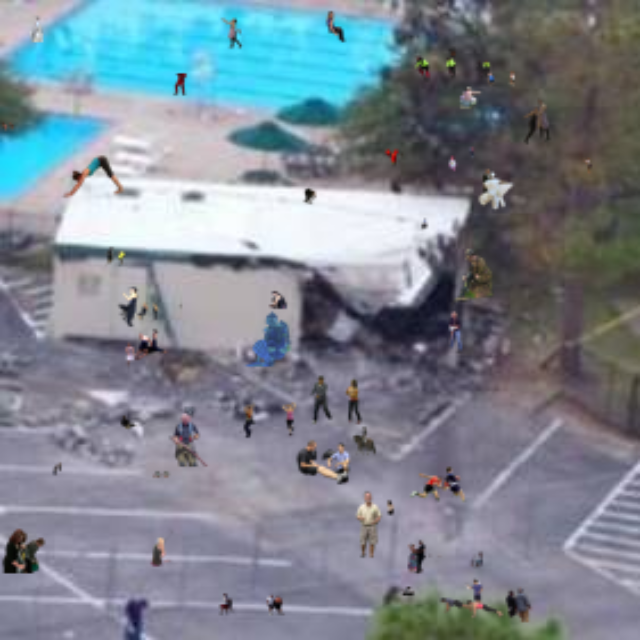
\includegraphics[width=\linewidth,height=3.6cm,keepaspectratio]{figures/arch_input.png}\\[2pt]
    {\small (a) input ($640\times640$)}
  \end{minipage}\hfill
  \begin{minipage}{0.44\linewidth}\centering
    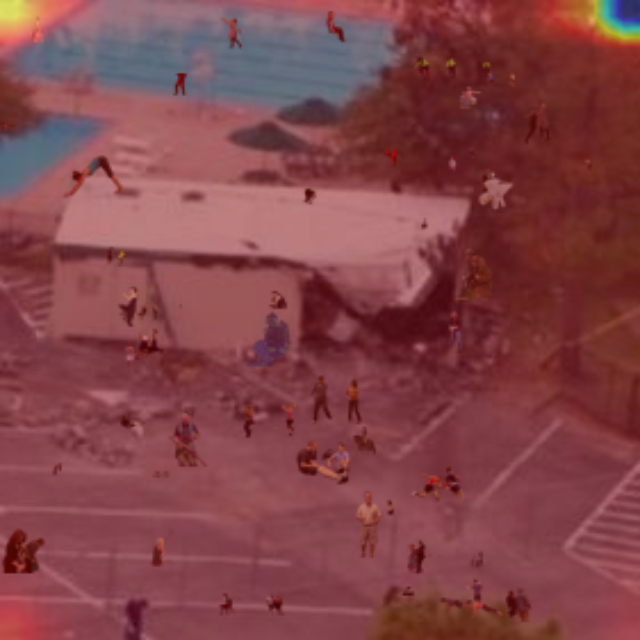
\includegraphics[width=\linewidth,height=3.6cm,keepaspectratio]{figures/cbam_overlay.png}\\[2pt]
    {\small (b) CBAM spatial attention}
  \end{minipage}\\[8pt]
  \begin{minipage}{0.44\linewidth}\centering
    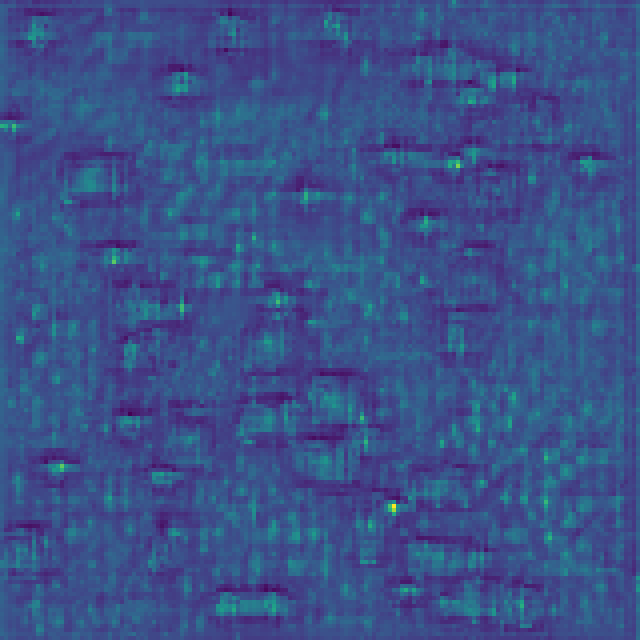
\includegraphics[width=\linewidth,height=3.6cm,keepaspectratio]{figures/p2_featuremap.png}\\[2pt]
    {\small (c) P2 feature response (stride 4)}
  \end{minipage}\hfill
  \begin{minipage}{0.44\linewidth}\centering
    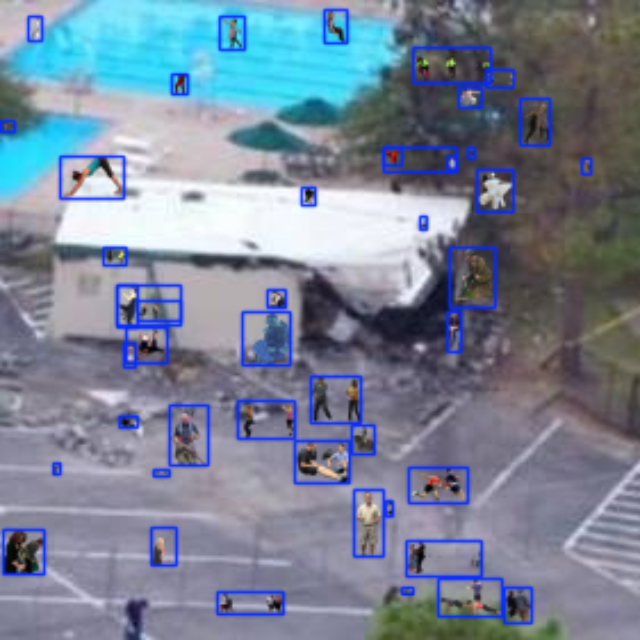
\includegraphics[width=\linewidth,height=3.6cm,keepaspectratio]{figures/arch_detections.png}\\[2pt]
    {\small (d) detections}
  \end{minipage}
  \caption{Trained detector on the running-example scene.}
  \label{fig:explain}
\end{figure}

\section{Architecture Novelties}
The design does not chase novelty for its own sake; each departure from the
baseline answers a specific failure mode of small-target detection, and each is
verified in isolation by the ablation of Chapter~IV. Three design decisions
define the contribution.

\subsection{Attention That Pays for Itself}
Aerial disaster scenes are dominated by distractors: rubble textures, water
glare, and vegetation produce strong generic feature responses that drown out
faint human signatures. The first design decision replaces the baseline's two
heavy C2PSA self-attention blocks with a single CBAM module. The intended effect
is illustrated in Figure~\ref{fig:cbameffect} together with the model's real
attention map: background clutter is down-weighted while the faint target
response is amplified. Because the substitution removes more parameters than it
adds, the attention improvement arrives at a negative parameter cost, about one
million parameters below the baseline, with the lowest latency of all evaluated
configurations.

\begin{figure}[H]
  \centering
  \figorplaceholder{figures/figures_png_format/cbam_effect.png}{6.5cm}
  \caption{Effect of the CBAM substitution on clutter and target response.}
  \label{fig:cbameffect}
\end{figure}

\subsection{A Detection Scale Where the Targets Are}
\label{sec:p2novel}
The second decision follows from the geometry in Figure~\ref{fig:strideprob}. A
detection cell summarises a stride-sized pixel region, so a $\sim$12-px human
occupies less than half of one P5 cell and under one P4 cell; even at P3 it spans
only about 1.5 cells. The added stride-4 scale is the first level at which such a
target covers about three cells, enough spatial support to be localised
precisely. On the C2A test split, $99.6\%$ of the human instances are smaller
than 32~px (Figure~\ref{fig:sizedist}), so the added level is not a marginal
refinement: it is the scale at which almost the entire dataset lives. The
branch is additive, and the existing P3--P5 pathway is left untouched, which is
what allows the ablation to attribute the very-tiny-recall gain to this single
change.

\begin{figure}[H]
  \centering
  \figorplaceholder{figures/figures_png_format/stride_problem.png}{7.5cm}
  \caption{Stride problem motivating the P2 head.}
  \label{fig:strideprob}
\end{figure}

\subsection{Single-Variable Additive Design}
The third decision is methodological. The four configurations evaluated in this
thesis are summarised in Table~\ref{tab:variants}: each row introduces exactly
one change with respect to the preceding design, so that the effect of attention
(CBAM), of the high-resolution detection scale (P2), of their combination, and
of the state-space neck can each be isolated. All configurations are trained on
the same frozen C2A split with identical optimisation settings (AdamW,
$\text{lr}_0 = 0.001$, cosine schedule, up to 300 epochs with early stopping)
and evaluated with the same protocol and thresholds, so that every reported
difference is attributable to the architectural change alone. This design is
what makes the negative state-space result interpretable: the variant fails
under conditions in which the P2 head demonstrably succeeds.

\begin{table}[H]
  \centering
  \caption{Additive ablation configurations, one change per step.}
  \label{tab:variants}
  \begin{tabular}{@{}l l l l@{}}
    \toprule
    \textbf{Configuration} & \textbf{Backbone attention} & \textbf{Detection scales} & \textbf{Neck} \\
    \midrule
    YOLO11m (baseline)   & C2PSA            & P3, P4, P5         & C3k2 \\
    + CBAM               & CBAM             & P3, P4, P5         & C3k2 \\
    + CBAM + P2          & CBAM             & P2, P3, P4, P5     & C3k2 \\
    + Mamba + CBAM + P2  & CBAM             & P2, P3, P4, P5     & C3k2Mamba (6 layers) \\
    \bottomrule
  \end{tabular}
\end{table}

\section{Loss Function Design}
\label{sec:loss3}
Training uses the standard YOLO11 composite detection loss, unchanged across all
four configurations so that the ablation compares architectures rather than
objectives. Predictions are matched to ground truth by the task-aligned
assigner, which scores each candidate cell by a product of its classification
confidence and its localisation quality, so that the cells that are best able to
both recognise and localise a target receive its supervision. Three terms are
then optimised.

Classification uses binary cross-entropy on the single \emph{person} class,
\begin{equation}
  \mathcal{L}_{\mathrm{cls}} = -\big[\, y \log \hat{p} + (1-y)\log(1-\hat{p}) \,\big],
\end{equation}
where $\hat{p}$ is the predicted objectness-class probability and $y$ the
assigned label. Box regression uses the complete-IoU loss,
\begin{equation}
  \mathcal{L}_{\mathrm{CIoU}} = 1 - \mathrm{IoU}
      + \frac{\rho^2(\mathbf{b}, \mathbf{b}^{gt})}{c^2} + \alpha v,
  \qquad
  v = \frac{4}{\pi^2}\Big(\arctan\tfrac{w^{gt}}{h^{gt}} - \arctan\tfrac{w}{h}\Big)^{\!2},
\end{equation}
where $\rho$ is the centre distance, $c$ the diagonal of the smallest enclosing
box, and $\alpha = v / \big((1-\mathrm{IoU}) + v\big)$ balances the aspect-ratio
term. The overlap, centre, and shape terms together matter for very small boxes,
whose IoU alone is unstable under sub-pixel shifts. Finally, box edges are
predicted as discrete distributions over binned offsets, trained with the
distribution focal loss,
\begin{equation}
  \mathcal{L}_{\mathrm{DFL}} = -\big[(y_{i+1}-y)\log S_i + (y-y_i)\log S_{i+1}\big],
\end{equation}
which sharpens the predicted distribution around the continuous target offset
$y$ that falls between bins $y_i$ and $y_{i+1}$. The total objective is the
weighted sum
\begin{equation}
  \mathcal{L} = \lambda_{\mathrm{box}} \mathcal{L}_{\mathrm{CIoU}}
              + \lambda_{\mathrm{dfl}} \mathcal{L}_{\mathrm{DFL}}
              + \lambda_{\mathrm{cls}} \mathcal{L}_{\mathrm{cls}},
\end{equation}
with the framework defaults $\lambda_{\mathrm{box}} = 7.5$,
$\lambda_{\mathrm{dfl}} = 1.5$, and $\lambda_{\mathrm{cls}} = 0.5$. The heavy
box weighting suits this task: with a single class, the difficulty is not
deciding \emph{what} an object is but \emph{where} a few-pixel target sits. The
added P2 level contributes its own predictions to all three terms exactly as
the standard levels do, so no loss re-balancing is needed when the scale is
added.

\section{Inference-Time Enhancement: SAHI and TTA}
Beyond the trained architecture, two inference-time procedures are evaluated as
optional operating modes; both leave the trained weights untouched and trade
latency for recall on the smallest targets. Their quantitative effect is
reported in Chapter~IV.

Slicing-aided hyper inference (SAHI) runs the detector over overlapping tiles of
the input so that very small targets occupy a larger fraction of each forward
pass (Figure~\ref{fig:sahipipe}). The image is sliced into square tiles (256 to
640~px, overlap 25--30\%) alongside one full-image pass; the detector runs on
each tile at a low confidence floor, and the per-tile detections are merged by
greedy non-maximum merging with an intersection-over-smaller matching metric at
threshold 0.5, which suits partially-cut boxes at tile borders.

\begin{figure}[H]
  \centering
  \figorplaceholder{figures/figures_png_format/sahi.png}{9.5cm}
  \caption{SAHI inference pipeline.}
  \label{fig:sahipipe}
\end{figure}

Test-time augmentation (TTA) instead re-runs the detector on rescaled and
flipped copies of the full image, at scale factors 1.0, 0.83, and 0.67, each
with a horizontal flip, and merges the union of predictions with standard NMS
(Figure~\ref{fig:ttapipe}). Because the model is fully convolutional, it can be
evaluated at a higher input resolution than it was trained at; running TTA at
1280~px doubles the effective resolution of the smallest targets. Chapter~IV
shows this is the most effective single inference-time setting, though the gain
collapses beyond twice the training resolution.

The two procedures buy recall in different ways and at different costs. SAHI
multiplies the number of forward passes by the tile count, so its latency grows
with the slicing density; its strength is that each tile is processed at close
to the training resolution, which is what lets it recover the smallest and most
occluded targets along cluttered edges. Test-time augmentation instead runs a
fixed handful of passes at a few scales, so its cost is bounded and predictable,
and its gain comes mainly from the single high-resolution pass rather than from
tiling. Because neither procedure alters the trained weights, both can be
switched on or off at deployment time according to the latency budget an
operator can afford: a ground station reviewing footage after a sortie can pay
for SAHI, while a live on-board feed may allow only the cheaper augmentation
pass or none at all. Chapter~IV quantifies the recall each setting adds and the
latency each costs, so the operating point can be chosen against a concrete
budget rather than by rule of thumb.

\begin{figure}[H]
  \centering
  \figorplaceholder{figures/figures_png_format/tta.png}{8cm}
  \caption{Test-time augmentation pipeline.}
  \label{fig:ttapipe}
\end{figure}

\section{Conclusion}
This chapter presented the proposed detector as an additive refinement of
YOLO11m: CBAM attention in place of C2PSA, a high-resolution P2 detection scale
for very small targets, and an explored state-space neck variant. The
architecture was specified to the layer level, the rationale for each novelty
was tied to a measurable failure mode, the unchanged composite loss keeps the
ablation interpretable, and two inference-time procedures extend the operating
envelope without retraining. The next chapter reports the experimental setup and
the quantitative and qualitative results of this design.
